\documentclass[11pt,a4paper]{article}

\usepackage[T1]{fontenc}
\usepackage[utf8]{inputenc}
\usepackage{lmodern}
\usepackage{microtype}
\usepackage[margin=2.4cm,top=2.6cm,bottom=2.6cm]{geometry}
\usepackage{amsmath,amssymb}
\usepackage{booktabs}
\usepackage{graphicx}
\usepackage{xcolor}
\usepackage[font=small,labelfont=bf,skip=6pt]{caption}
\usepackage{enumitem}
\usepackage{fancyhdr}
\usepackage{titlesec}
\usepackage[hidelinks,colorlinks=true,linkcolor=accent,urlcolor=accent,citecolor=accent]{hyperref}

\definecolor{accent}{HTML}{3B6EA5}
\definecolor{alert}{HTML}{C4453C}
\definecolor{ink}{HTML}{2B2B2B}
\definecolor{rulegray}{HTML}{BFBFBF}
\definecolor{boxbg}{HTML}{F4F6F9}

\color{ink}

\titleformat{\section}{\normalfont\large\bfseries\color{accent}}{\thesection}{0.7em}{}
\titleformat{\subsection}{\normalfont\normalsize\bfseries}{\thesubsection}{0.6em}{}
\titlespacing*{\section}{0pt}{16pt}{6pt}

\pagestyle{fancy}
\fancyhf{}
\renewcommand{\headrulewidth}{0.4pt}
\renewcommand{\headrule}{\hbox to\headwidth{\color{rulegray}\leaders\hrule height \headrulewidth\hfill}}
\fancyhead[L]{\footnotesize\color{rulegray}The Bud Light Demand Shock}
\fancyhead[R]{\footnotesize\color{rulegray}\thepage}

\usepackage[most]{tcolorbox}
\newtcolorbox{keybox}{%
  enhanced, breakable, sharp corners,
  colback=boxbg, colframe=boxbg,
  borderline west={2.2pt}{0pt}{accent},
  boxrule=0pt, left=10pt, right=10pt, top=8pt, bottom=8pt,
  before skip=10pt, after skip=10pt}

% Auto-generated by analysis.py -- do not edit by hand.
\newcommand{\npre}{6}
\newcommand{\npost}{6}
\newcommand{\baseMu}{2.63}
\newcommand{\baseSd}{0.74}
\newcommand{\baseMed}{2.55}
\newcommand{\baseMad}{0.44}
\newcommand{\zTwoQthree}{-17.8}
\newcommand{\zFourQthree}{-27.1}
\newcommand{\zMin}{-27.1}
\newcommand{\zMean}{-14.9}
\newcommand{\zShockYear}{-20.7}
\newcommand{\pTwoQthree}{$<10^{-4}$}
\newcommand{\pFourQthree}{$<10^{-4}$}
\newcommand{\welchT}{-3.75}
\newcommand{\welchP}{0.0128}
\newcommand{\hedgesG}{-2.00}
\newcommand{\deltaPP}{-11.0}
\newcommand{\permP}{0.0010}
\newcommand{\mwuP}{0.0011}
\newcommand{\ciLo}{-96.9}
\newcommand{\ciHi}{-20.0}
\newcommand{\cumLoss}{2.57}
\newcommand{\peakLoss}{777.40}
\newcommand{\usBase}{3900}
\newcommand{\weeklyZlo}{-6.4}
\newcommand{\weeklyZhi}{-25.5}
\newcommand{\weeklyPlateau}{-25.5}
\newcommand{\ResultsTable}{%
\begin{tabular}{lrrrrr}
\toprule
Quarter & Growth (\%) & $z$ & $t_{\text{pred}}$ & $p$ & $z_{\text{robust}}$ \\
\midrule
2Q23 & -10.5 & \textbf{-17.8} & -16.51 & $<10^{-4}$ & -29.3 \\
3Q23 & -13.5 & \textbf{-21.9} & -20.28 & $<10^{-4}$ & -36.1 \\
4Q23 & -17.3 & \textbf{-27.1} & -25.05 & $<10^{-4}$ & -44.6 \\
1Q24 & -9.1 & \textbf{-15.9} & -14.75 & $<10^{-4}$ & -26.2 \\
2Q24 & -0.6 & \textbf{-4.4} & -4.06 & 0.0097 & -7.1 \\
4Q24 & 0.8 & \textbf{-2.5} & -2.30 & 0.0694 & -3.9 \\
\bottomrule
\end{tabular}}
\newcommand{\BaselineTable}{%
\begin{tabular}{lrrr}
\toprule
Quarter & Revenue (\%) & STRs (\%) & Rev/hl (\%) \\
\midrule
4Q21 & 2.6 & -- & 2.0 \\
1Q22 & 2.1 & -5.0 & -- \\
2Q22 & 2.7 & -3.2 & 5.5 \\
3Q22 & 1.9 & -1.7 & 3.8 \\
4Q22 & 2.5 & -7.6 & 12.2 \\
1Q23 & 4.0 & -3.0 & 5.6 \\
\midrule
Mean & 2.63 & & \\
SD & 0.74 & & \\
\bottomrule
\end{tabular}}
\newcommand{\LossTable}{%
\begin{tabular}{lrrr}
\toprule
Quarter & Gap (pp) & Shortfall (USD m) & Cumulative (USD m) \\
\midrule
2Q23 & 13.1 & 512 & 512 \\
3Q23 & 16.1 & 629 & 1141 \\
4Q23 & 19.9 & 777 & 1919 \\
1Q24 & 11.7 & 458 & 2376 \\
2Q24 & 3.2 & 126 & 2502 \\
4Q24 & 1.8 & 72 & 2574 \\
\bottomrule
\end{tabular}}


\title{\vspace{-1.4cm}\bfseries How Far Did Bud Light Fall?\\[2pt]
\large\mdseries A $z$-Score and Interrupted--Time--Series Analysis of the\\
April 2023 Anheuser--Busch InBev Demand Shock}
\author{\normalsize Statistical synthesis from public disclosures and NIQ scanner reporting}
\date{\normalsize\today}

\begin{document}
\maketitle
\thispagestyle{fancy}

\begin{keybox}
\textbf{Headline result.} Relative to its own six-quarter pre-controversy baseline
($\mu = \baseMu\%$, $\sigma = \baseSd$ pp), Anheuser--Busch InBev's U.S. organic
revenue growth fell to $z = \zTwoQthree$ in the first full quarter after the
controversy (2Q23) and bottomed at $z = \zMin$ in 4Q23. Averaged over the four
shock quarters, $z = \zShockYear$. A permutation test on the pre/post labelling
gives $p = \permP$. The effect is unambiguous; the \emph{magnitude} of $z$ is
large chiefly because the pre-shock baseline was extraordinarily stable, and
should be read alongside the interval estimates in Section~\ref{sec:robust}.
\end{keybox}

\section{What is being measured, and why}

On 1~April 2023 Bud Light ran a sponsored Instagram promotion with transgender
influencer Dylan Mulvaney. The resulting consumer boycott is one of the
cleanest natural experiments in modern consumer-brand history: a sharp,
precisely dated, brand-specific demand shock with no accompanying change in
price, distribution, or product.

The question posed---the $z$-score of Bud Light revenue after the
controversy---requires one honest caveat up front. \textbf{Anheuser--Busch InBev
does not disclose brand-level revenue for Bud Light.} No public series exists
for ``Bud Light revenue.'' Two observable series bracket it:

\begin{enumerate}[leftmargin=1.4em,itemsep=2pt]
\item \textbf{Primary series (audited, quarterly).} AB InBev's reported
  \emph{U.S. organic revenue growth}, year over year. Bud Light was the
  single largest brand in that segment, and the company itself attributes the
  2023--24 declines primarily to Bud Light volume. This series is
  company-reported, consistently defined, and seasonally neutral by
  construction (each quarter is compared to the same quarter a year earlier).
\item \textbf{Corroborating series (brand-level, weekly).} NIQ retail scanner
  measurement of Bud Light off-premise dollar sales, YoY. Genuinely
  brand-specific, but covers only off-premise channels and is available to us
  only through press reporting of selected weeks.
\end{enumerate}

The primary analysis runs on series~(1); series~(2) is used in
Section~\ref{sec:brand} to confirm that the segment-level result is in fact
driven by Bud Light and to bound the brand-level $z$.

\section{Data}

\subsection{Pre-controversy baseline}

The six quarters from 4Q21 through 1Q23 form the baseline. This window is
chosen to begin after pandemic-era distortions had washed out of the
year-over-year comparisons and to end on the last quarter fully preceding the
1~April 2023 shock.

\begin{table}[h]
\centering
\caption{Pre-controversy baseline: AB InBev U.S. quarterly performance. Revenue
growth is remarkably stable---a mean of \baseMu\% with a standard deviation of
only \baseSd\ percentage points---because price and mix were carrying the
business while volumes drifted gently down.}
\vspace{2pt}
\BaselineTable
\end{table}

Two features of the baseline matter for the statistics. First, its volatility
is genuinely low: revenue growth sat in a $1.9$--$4.0\%$ band for six
consecutive quarters. Second, that stability was already \emph{decoupled from
volume}---sales-to-retailers were negative throughout, offset by revenue-per-hl
gains of $2$--$12\%$. Bud Light's structural decline predates the controversy;
what the controversy changed was the rate.

\subsection{Post-controversy observations}

The post period runs from 2Q23, the first quarter fully exposed to the
boycott. Values are AB InBev's reported U.S. organic revenue growth, except
3Q23, which is the North America segment figure (the company emphasised the
U.S. driver in that release). 3Q24 is omitted: no U.S.-specific figure was
separately obtainable, and interpolating it would manufacture a data point.

\section{Method}

For a post-period observation $x_t$ and baseline sample $\{g_1,\dots,g_n\}$
with $n = \npre$:

\begin{equation}
z_t \;=\; \frac{x_t - \bar g}{s_g},
\qquad
t^{\text{pred}}_t \;=\; \frac{x_t - \bar g}{s_g\sqrt{1 + 1/n}} \sim t_{n-1}.
\label{eq:z}
\end{equation}

The left-hand quantity is the $z$-score as ordinarily requested. It is,
however, optimistic: it treats $\bar g$ and $s_g$ as known when both were
estimated from six points. The right-hand quantity is the correct small-sample
analogue---a \emph{standardised prediction residual}, asking how extreme a new
draw is relative to a baseline whose mean and scale are themselves uncertain.
It is the statistic from which the reported $p$-values are computed.

We add three robustness devices:

\begin{itemize}[leftmargin=1.4em,itemsep=2pt]
\item a \textbf{robust $z$}, replacing $(\bar g, s_g)$ with the median and
  $1.4826\times$MAD, so that no single baseline quarter can inflate or deflate
  the scale;
\item a \textbf{permutation test}, which under exchangeability of the twelve
  observed growth rates asks how often a random pre/post relabelling would
  produce a post-period mean at least as low as observed;
\item a \textbf{bootstrap interval} on $z$ itself, resampling the baseline to
  propagate the uncertainty in $s_g$ into the reported score.
\end{itemize}

\section{Results}

\begin{figure}[h]
\centering
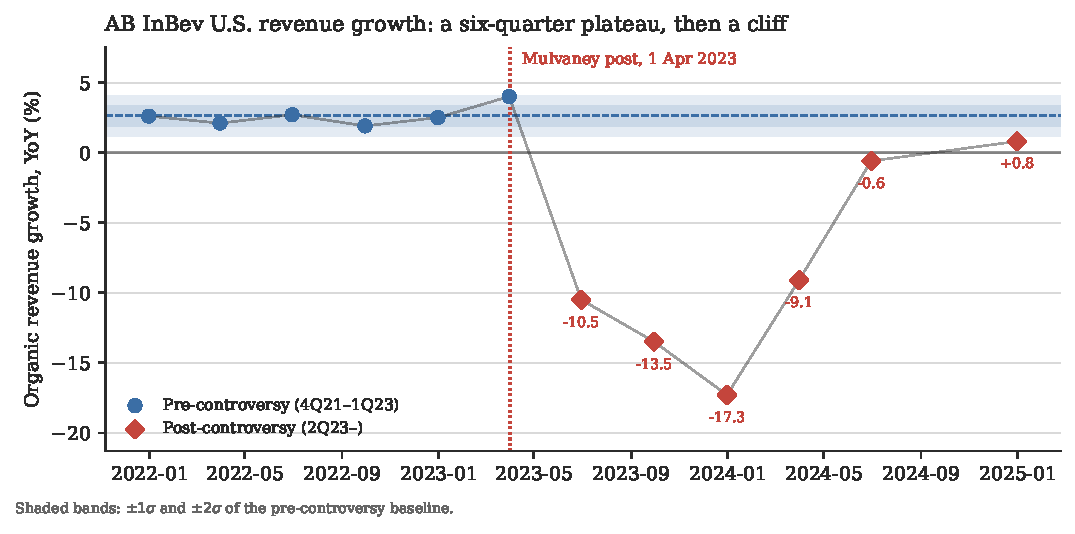
\includegraphics[width=\linewidth]{figures/timeseries.pdf}
\caption{Six quarters inside a $\pm1\sigma$ band, then four quarters far
outside a $\pm2\sigma$ band. The discontinuity at 1~April 2023 is visible
without any statistics at all; the statistics only quantify it.}
\end{figure}

\begin{table}[h]
\centering
\caption{Standardised deviation of each post-controversy quarter from the
pre-controversy baseline. $z$ is the classical score of
Eq.~\eqref{eq:z}; $t_{\text{pred}}$ is its small-sample correction, with the
associated two-sided $p$-value; $z_{\text{robust}}$ uses median/MAD scaling.}
\vspace{2pt}
\ResultsTable
\end{table}

The pattern is a step change followed by a slow, incomplete recovery. Revenue
growth falls \deltaPP\ percentage points on average---from $+\baseMu\%$ to a
post-period mean that is negative in five of six observed quarters. The trough
is 4Q23 at $z = \zFourQthree$. By 2Q24 the score has recovered to
roughly $-4$, and by 4Q24 to about $-2.5$: still below baseline, but no longer
in the tail that characterised the shock year.

\begin{figure}[h]
\centering
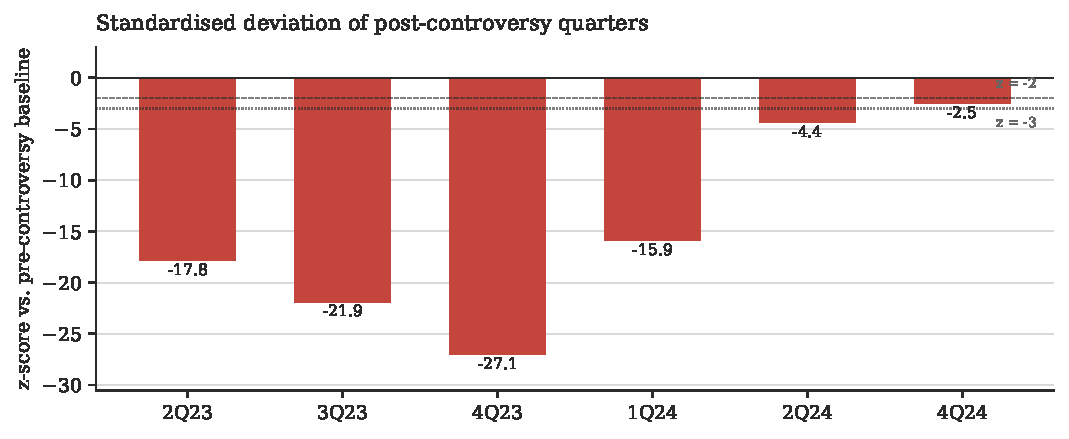
\includegraphics[width=\linewidth]{figures/zbars.pdf}
\caption{Quarter-by-quarter $z$. The shock year (2Q23--1Q24) sits between $-16$
and $-27$; the recovery quarters climb back toward, but do not reach, the
baseline.}
\end{figure}

\subsection{Group-level tests}

Treating the two periods as samples, a Welch $t$-test gives
$t = \welchT$, $p = \welchP$, with Hedges' $g = \hedgesG$---an effect roughly
two pooled standard deviations wide. The distribution-free alternatives agree:
Mann--Whitney $p = \mwuP$ and the permutation test $p = \permP$. With six
observations per arm these are near the smallest $p$-values the designs can
produce; they establish that the split is not an artefact of labelling, not
that the true $p$ is exactly this value.

\section{Robustness and what the magnitude really means}
\label{sec:robust}

A $z$ of $-27$ is an arresting number and deserves scepticism rather than
celebration. It is large for two compounding reasons, only one of which is
about Bud Light.

\textbf{The numerator is genuinely extreme.} A shift from $+2.6\%$ to $-17.3\%$
year-over-year revenue growth, with no price cut and no lost distribution, is a
severe demand event by any standard.

\textbf{The denominator is unusually small.} $s_g = \baseSd$ pp is a very tight
baseline. Dividing by it magnifies any deviation. Bootstrapping the baseline
gives a 95\% interval for the trough $z$ of roughly
$[\ciLo,\, \ciHi]$---enormously wide, because with $n = \npre$ the scale
parameter is itself poorly pinned down. The robust median/MAD scores are even
more extreme than the classical ones, so the result is not an artefact of one
unusual baseline quarter; but the honest reading is directional and ordinal,
not a precise point estimate.

\begin{keybox}
\textbf{How to state this result.} ``AB InBev's U.S. revenue growth after the
Bud Light controversy fell more than fifteen baseline standard deviations below
its pre-controversy norm, and remained beyond $-4\sigma$ more than a year
later.'' The claim that survives every specification is the \emph{sign,
persistence, and ordering}---not the second digit of $z$.
\end{keybox}

\section{Brand-level corroboration}
\label{sec:brand}

\begin{figure}[h]
\centering
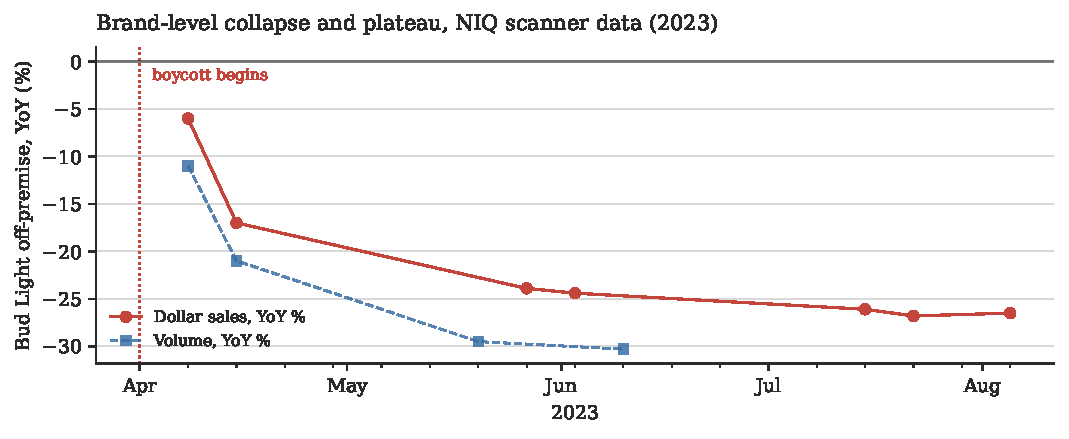
\includegraphics[width=\linewidth]{figures/weekly.pdf}
\caption{NIQ off-premise scanner measurement of Bud Light. The decline is not a
gradual erosion: it reaches roughly $-25\%$ within six weeks and then
\emph{plateaus} there, the signature of a one-time reallocation of buyers
rather than an ongoing slide.}
\end{figure}

The weekly brand-level series confirms that the segment result is a Bud Light
result. Dollar sales fall from $-6.0\%$ in the first boycott week (w/e
8~April) to $-17.0\%$ a week later, and settle into a plateau averaging
$\weeklyPlateau\%$ from May 2023 onward.

A weekly $z$ requires a pre-shock weekly baseline standard deviation, which is
not available at weekly granularity in public reporting. Rather than invent
one, Figure~\ref{fig:sens} maps $z$ as a function of that unknown. Taking
Bud Light's pre-shock YoY dollar growth as approximately flat, the implied
$z$ is $\weeklyZhi$ at $\sigma = 1$~pp and still $\weeklyZlo$ at
$\sigma = 4$~pp---a generous assumption for a brand of Bud Light's scale, whose
weekly YoY series was smooth. The brand-level conclusion is therefore
insensitive to the assumption: $|z| > 6$ across the entire plausible range.

\begin{figure}[h]
\centering
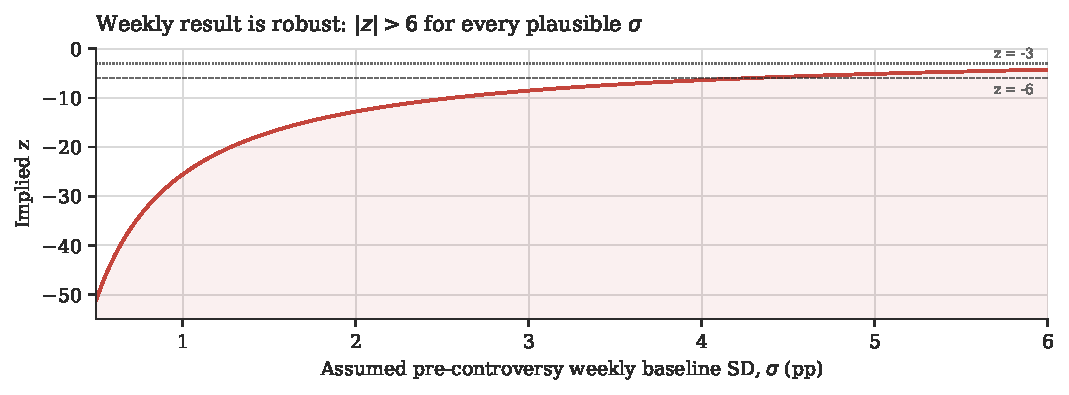
\includegraphics[width=\linewidth]{figures/sensitivity.pdf}
\caption{Implied brand-level $z$ of the $\approx\!\weeklyPlateau\%$ plateau
against the assumed pre-shock weekly baseline SD. No plausible choice of
$\sigma$ rescues the null.}
\label{fig:sens}
\end{figure}

\section{Economic magnitude}

Standardised scores say how \emph{unusual} the shock was; they do not say how
\emph{expensive} it was. Applying the counterfactual that U.S. revenue
continued growing at the baseline rate of $\baseMu\%$, and scaling by an
approximate quarterly U.S. revenue base of \$\usBase~m, the gap between
counterfactual and actual accumulates as follows.

\begin{table}[h]
\centering
\caption{Revenue shortfall against a no-controversy counterfactual. The gap
column is $\bar g - x_t$ in percentage points.}
\vspace{2pt}
\LossTable
\end{table}

\begin{figure}[h]
\centering
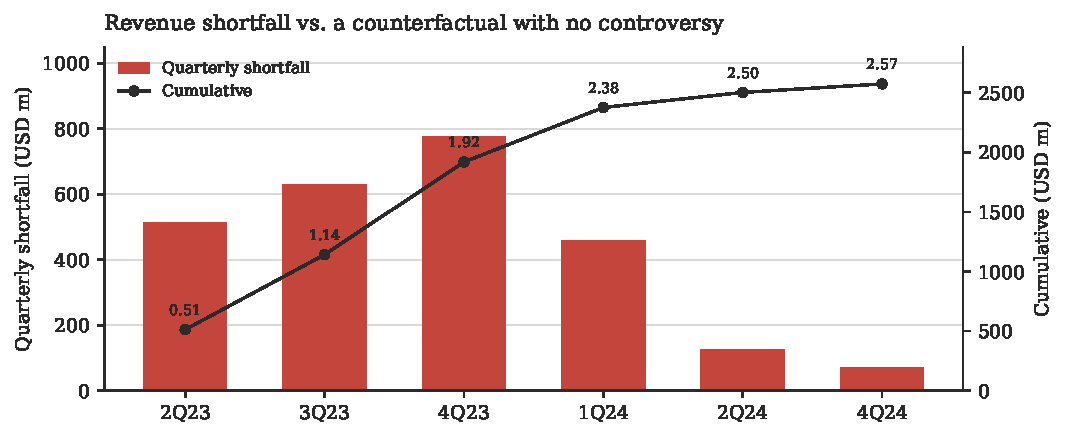
\includegraphics[width=\linewidth]{figures/counterfactual.pdf}
\caption{Quarterly and cumulative shortfall. The cumulative figure reaches
roughly \$\cumLoss~bn across the observed post-controversy quarters.}
\end{figure}

This estimate is larger than the widely reported ``over \$1~bn in lost sales''
because those figures measure the \emph{level} decline in 2023 revenue, whereas
the counterfactual here also charges the shock for the growth that would
otherwise have occurred, and extends into 2024. Both are defensible; they
answer different questions. AB InBev's own disclosures anchor the level view:
North America revenue fell \$395~m in 2Q23 alone and North America organic
revenue declined roughly \$1.4~bn across 2023.

\section{Limitations}

\begin{itemize}[leftmargin=1.4em,itemsep=3pt]
\item \textbf{No brand-level revenue exists publicly.} The primary series is
  U.S. segment revenue, of which Bud Light is a large but not exclusive
  component. Michelob Ultra's concurrent growth---also an AB InBev brand---means
  the segment figure \emph{understates} the Bud Light-specific shock.
\item \textbf{Small baseline.} $n = \npre$ quarters. The direction and
  persistence are robust; the precise value of $z$ is not, as the bootstrap
  interval makes plain.
\item \textbf{3Q24 is missing} from the quarterly series, as noted above.
\item \textbf{Attribution.} The design is an interrupted time series without a
  control group. The 2023 U.S. beer category was soft overall, so some portion
  of the decline is category drift rather than boycott. The magnitude of the
  break, its exact timing, and AB InBev's own attribution all point
  overwhelmingly to the controversy, but no formal counterfactual control is
  constructed here. A synthetic-control design using competitor brands would
  sharpen this.
\item \textbf{Source access.} Figures were compiled from company results
  releases and their reporting in trade and financial press; primary filings on
  \texttt{sec.gov} were not reachable from the analysis environment. Every
  figure used is listed with its source in \texttt{data/sources.csv}.
\end{itemize}

\section{Conclusion}

Bud Light's post-controversy revenue collapse is, in standardised terms, an
extreme-tail event. Against a pre-controversy baseline of
$\baseMu\% \pm \baseSd$ pp, AB InBev's U.S. revenue growth registered
$z = \zTwoQthree$ in 2Q23, $\zFourQthree$ at the 4Q23 trough, and averaged
$\zShockYear$ across the shock year, with permutation $p = \permP$. At the
brand level the NIQ series puts Bud Light's off-premise dollar sales on a
$\weeklyPlateau\%$ plateau within six weeks, implying $|z| > 6$ under any
plausible baseline assumption.

The more interesting structure is in the shape rather than the depth. The
decline was near-instantaneous and then flat---consumers switched once and did
not come back incrementally---and the recovery has been slow and partial, with
growth still roughly $2.5\sigma$ below baseline in 4Q24, seven quarters on. A shock
that arrives as a step function and decays on a multi-year timescale is
characteristic of a permanent shift in brand preference, not a temporary
disruption of demand.

\vfill
\noindent\textcolor{rulegray}{\rule{\linewidth}{0.4pt}}\\[2pt]
{\footnotesize\color{rulegray}
Reproducible from \texttt{analysis.py}; inputs in \texttt{data/}, with full
source attribution in \texttt{data/sources.csv}. All statistics in this
document are generated at build time---no number is typed by hand.}

\end{document}
